\documentclass {article}
\usepackage[margin=1.0in]{geometry}
\usepackage[style=mla-new]{biblatex}
\usepackage[hidelinks]{hyperref}
\usepackage{graphicx}
\usepackage{titlesec}
\titlespacing*{\section}{0pt}{3ex plus .5ex minus .2ex}{0ex}
\addbibresource{sources.bib}
\newcommand{\sechint}[1]{\small{\emph{#1}} \bigskip}

\begin{document}
\begin{titlepage}
	\centering
	
\includegraphics[width=0.8\textwidth]{images/umd_logo.jpg} \\ \bigskip
	\LARGE{Electrical and Computer Engineering Department \\University of Massachusetts Dartmouth}\\
	\bigskip 
	\LARGE{Master's of Science \\ Thesis Proposal -- Second Draft} \\
	\bigskip 
	\Huge{\bf Viral Certificate Revocation List Distribution for VANET} \\ \medskip
	\LARGE{\bf By Robert Mushrall III}

	\vfill
	\begin{table}[!hb]
		\centering
		\begin{tabular}{ l l }
			\line(1,0){250} & \line(1,0){150} \\
			\small{Robert Mushrall III}  & \small{Date} \\
			\small{Electrical and Computer Engineering Department} \\
			\small{M.S. Computer Engineering Student} & \\
			\vspace{.3cm} \\
			\line(1,0){250} & \line(1,0){150} \\
			\small{Dr. Hong Liu} & \small{Date} \\
			\small{Electrical and Computer Engineering Department} \\
			\small{Graduate Advisor} & \\
			\vspace{.3cm} \\
			\line(1,0){250} & \line(1,0){150} \\
			\small{Dr. Paul Fortier} & \small{Date} \\
			\small{Electrical and Computer Engineering Department} \\
			\small{Graduate Committee} & \\
			\vspace{.3cm} \\
			\line(1,0){250} & \line(1,0){150} \\
			\small{Brian Hewett} & \small{Date} \\
			\small{Product Manager, General Dynamics Mission Systems} \\
			\small{Graduate Committee} & \\
		\end{tabular}
	\end{table}
	\thispagestyle{empty}
\end{titlepage}
\setcounter{page}{2}

\tableofcontents
\pagebreak

\section{Background}{\sechint{One paragraph (1/3 page) to orient the reader to the area of research.}}

With the number of vehicles on the road and the safety risks these vehicles (and their drivers) pose, new technology is needed to reduce accidents and improve travel in terms of congestion control and comfort. A VANET (Vehicular Ad-Hoc NETwork) will open up communication channels allowing helpful information to be passed between vehicles and alerting drivers of possible hazards or even adjusting routes to minimize travel time. This network will be possible with V2V (Vehicle to Vehicle) and V2I (Vehicle to Infrastructure) communication. V2V communication allows vehicles to pass information, such as speed and nearby dangers, between each other. V2I communication allows vehicles to communicate with an infrastructure that may provide extra benefits to a VANET.

While helpful information can be passed, vehicles may malfunction and attackers can ever cause vehicles to misbehave, which can negatively impact safety, counter to the very reason VANET exists. The Security Credential Management System (SCMS) is the leading solution to secure VANET communication. It includes components common to a Public Key Infrastructure, with the addition of several functions to account for the difference between a traditional network versus a VANET. There are two methods for removing malfunctioning or misbehaving vehicles, not provisioning certificates and adding their provisioned certificates to a Certificate Revocation List (CRL) so other vehicles know not to trust it.

Currently, the CRL distribution method is not yet finalized. The current method is for each vehicle to perform an HTTP GET request, which requires an active connection to the internet~\autocite{brecht_scms_nodate}. One method was proposed which included an ``epidemic distribution''~\autocite{haas_efficient_2011} which promises the ability to distribute CRLs across an urban area within hours of an update.

\section{Problem Statement}{\sechint{One or two sentences that concisely state the problem that will be addressed by the research.}}

The current method for distributing CRLs is not effective for vehicles that do not have an active internet connection. A method for distributing CRLs must be defined that allows updates to be quick, does not overload the finite resource used for V2V and V2I communication, and provides the widest dissemination possible.

\section{Technical Discussion}{\sechint{About one page that presents some of the more important aspects of the proposed research. This should include a summary of the state-of-the-art in the particular research area.}}

The highly dynamic nature of VANETs presents

\subsection{The Security Credential Mangement System}
Whyte, Weimerskirch, Kumar and Hehn propose SCMS, the V-PKI that this research will be focused on. This scheme is currently being finalized with the US Department of Transportation~\autocite{brecht_security_2018}. Figure~\ref{scms_overview} represents SCMS as a whole. 
\begin{figure}[!ht]
	\centering
	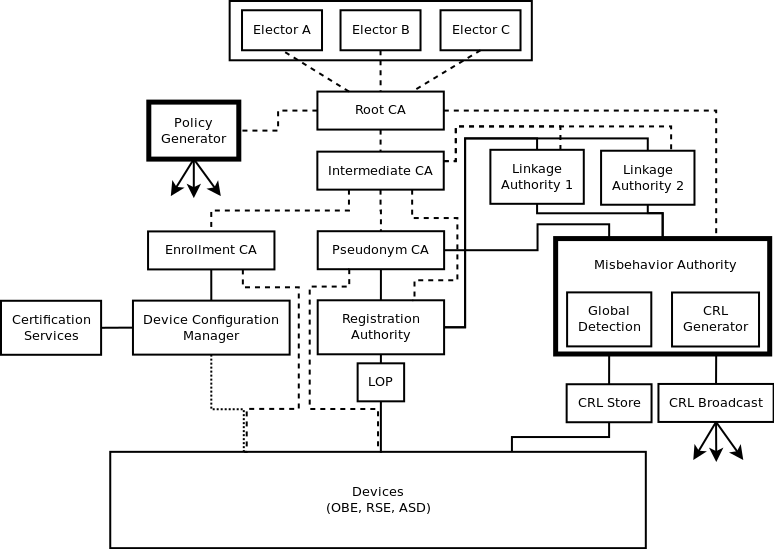
\includegraphics[width=.8\textwidth]{images/scms_diagram.png}
	\caption{SCMS Overview}
	\label{scms_overview}
\end{figure}
The trust within SCMS begins with the Root CA, which then trusts (shown by the dashed line) the Intermediate CA, the Policy Generator, and the Misbehavior Authority. In turn, the Intermediate CA trusts the Enrollment CA, the Pseudonym CA, the Registration Authority, and the linkage authorities. The end devices, such as the On Board Equipment (OBE), Road Side Equipment (RSE) and Aftermarket Safety Devices (ASD), are all trusted by the Enrollment CA and the Pseudonym CA. The electors vote on the Root CA. In the event the Root CA's private key is compromised or expired, the electors will vote on the new Root CA, and all necessary components and end devices will update their trust. The Policy Generator and the Misbehavior Authority intrinsically central (bolded), meaning that only one of these must exist for SCMS to function properly.
For privacy reasons, SCMS uses pseudonym certificates, which are certificates that vehicles use instead of a singular certificate. This helps obfuscate the sender of signed messages. To further protections against privacy, SCMS separates operations so that at least two operations need to be compromized before being able to track an individual vehicle. SCMS does not implement a Tamper Proof Device, like suggested Reya, et al. but this also means that SCMS does not rely on the trustworthiness of each particular vehicle. The authors state that one main challenge to their scheme is efficient certificate revocation while protecting drivers' privacy from attackers on the inside.

\subsection{Technical Challenges}

\subsection{Security Vulnerabilities}

\subsection{Proposed Solutions}

\section{Approach}{\sechint{One paragraph (1/3 page) that describes the methods that will be applied in conducting the research.}}

SCMS's effectiveness will be evaluated using simulations. The software that will be used is Veins (version 4.6), OMNet++ (version 5.1-2), and Sumo (version 0.30.0-1). OMNet++ is a network simulator that will be used to simulate the protocol and network stacks. This is where most of the V-PKI under test will be implemented. Veins will be used to simulate cars on a road system. This adds the complexity of moving cars in different directions and adds traffic scenarios. To tie the two together, Sumo will be used.
The programming language used will be C++ since that is the language OMNet++ supports, as well as the popularity of C++ in embedded environments such as where SCMS will likely by implemented. SCMS will be evaluated on three parts: confidentiality, integrity, and availability. Confidentiality will be gauged on the ability to protect vehicles privacy, both from inside attackers and outside attackers. Integrity will be gauged on the ability to prevent invalid information from being spread using authenticated messages. Since SCMS currently doesn't have misbehavior detection, this metric may assume misbehaving nodes and properly functioning nodes are already known. Availability will be measured by the computational overhead SCMS requires, as well as resilience to attacks.

\pagebreak
\section{Works Cited}
\printbibliography[title={\ }]

\pagebreak
\section{Schedule and Milestones}{\sechint{Displays a plan for completion of the project or thesis.}}

\begin{table}[!ht]
	\centering
	\begin{tabular}{l|c}
		\hline
		Task & Time \\ \hline \hline
		Updated Proposal Submitted & April 2018 \\ \hline
		Tests, Criteria Defined & May 2018 \\ \hline
		Simulations Completed & June 2018 \\ \hline
		Results Finalized & July 2018 \\ \hline
		Defense & Early August 2018 \\ \hline
		Submit Thesis & Mid August 2018 \\ \hline
	\end{tabular}
	\caption{Timeline}
\end{table}

\end{document}
